%!TEX root = main.tex
\section{Algorithms}
\subsection{Support Vector Regression}

As a one of machine learning algorithms to estimate time of a CAL module execution we will use \textit{Epsilon-Support Vector Regression}~\cite{svrc} (SVR) - it is based on Support Vector Machine (SVM, orginally named \textit{support-vector networks}\cite{svm}).

We will use SVR model with a RBF kernel\cite{rbf_kernel} which is the most known flexible kernel and it could project the features vectors into infinite dimensions. It uses Taylor expansion which is equivalent to use an infinite sum over the polynomial kernels. It allows to model any function that is a sum of unknown degree polynomials.

Using kernel, the resulting algorithm is formally similar, except that every dot product is replaced by a nonlinear kernel function. This allows the algorithm to fit the maximum-margin hyperplane in a transformed feature space. The RBF kernel have the following form:

\[ K_{RBF}(\vec{x}, \vec{x}') = \exp{(-\gamma||\vec{x} - \vec{x}'||)}\ \textnormal{, where:}\]
\begin{itemize}
	\item $ ||\vec{x} - \vec{x}'|| $ is the squared Euclidean distance between the two vectors of features,\newline
	\item $ \gamma $ - hyperparameter described in more details below.
\end{itemize}
In the SVR algorithm we are looking for a hyperplane \textit{y} in the following form:
\[ y = \vec{w} \vec{x} + b \textnormal{, where:}\]
\begin{itemize}
	\item $ \vec{x} $ - vector of features,
	\item $ \vec{w} $ - normal vector to the hyperplane \textit{y}, using a kernel the $ \vec{w} $ is also in the transformed space.
\end{itemize}
Training the original SVR means solving:
\[ \frac{1}{2}||w||^2  + C \sum_{i}^{N}(\xi_i+\xi_i^*) \textnormal{,}\]
with the following constraints:
\[ y_i - \vec{w}x_i - b \le \epsilon + \xi_i  \]
\[ -y_i + \vec{w}x_i + b \le \epsilon + \xi_i^*  \]
\[ \xi_i \xi_i^* \ge 0 \]
Figure~\ref{fig:svrc} shows the wanted hyperplane with marked \textit{$\xi$} and \textit{$\epsilon$} parameters.
As we already choosed the RBF kernel for the SVR algorithm, our modelling is simplified to just find the best values of the following hyperparameters\cite{svr}:
\begin{enumerate}
	\item \textit{C} -the weight of an error cost. The regularization\footnote{Regularization is a way to give a penalty to certain models (usually overly complex ones)} hyperparameer, have to be strictly positive. The example from the figure use l1 penalty (the library that we use to modelling use the squared epsilon-insensitive loss with l2 penalty). The strength of the regularization is inversely proportional to C. The larger value of C the more variance is introduced into the model. 
	\item \textit{epsilon} - It specifies the epsilon-tube within which no penalty is associated in the training loss function with points predicted within a distance epsilon from the actual value. As it is shown of the figure~\ref{fig:epsilon} the grey data points do not provide any penalty to the loss function because they are within the allowed epsilon range around the approximation\footnote{\label{figure_example}The figure is based on some example data and it only shows the hyperparameter influence on model.}.
	\item \textit{gamma} - The \textit{gamma} hyperparameter can be seen as the inverse of the radius of influence of samples selected by the model as support vectors. Increasing the value of \textit{gamma} hyperparameter causes the variance increase what is shown in the figure~\ref{fig:gamma}\footnotemark[\getcountref{figure_example}].
	
\end{enumerate}
\begin{figure}[!htb]
	\caption{Visualization of the SVR's epsilon parameter~\citeinside{epsilon}.}
	\centering
	\label{fig:epsilon}
	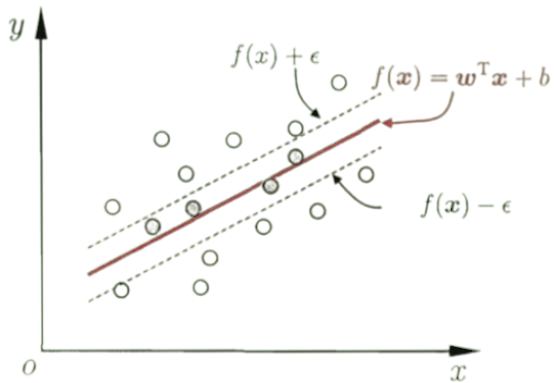
\includegraphics[width=0.45\textwidth]{epsilon}
\end{figure}
\begin{figure}[!htb]
	\caption{SVR's C parameter~\citeinside{svrc} influence on model.}
	\centering
	\label{fig:svrc}
	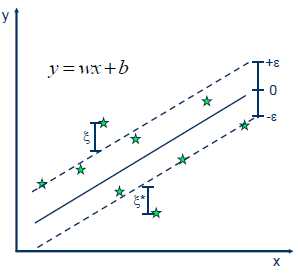
\includegraphics[width=0.45\textwidth]{svrC}
\end{figure}
\begin{figure}[!htb]
	\caption{SVR's gamma hyperparameter~\citeinside{gamma} influence on the model variance.}
	\centering
	\label{fig:gamma}
	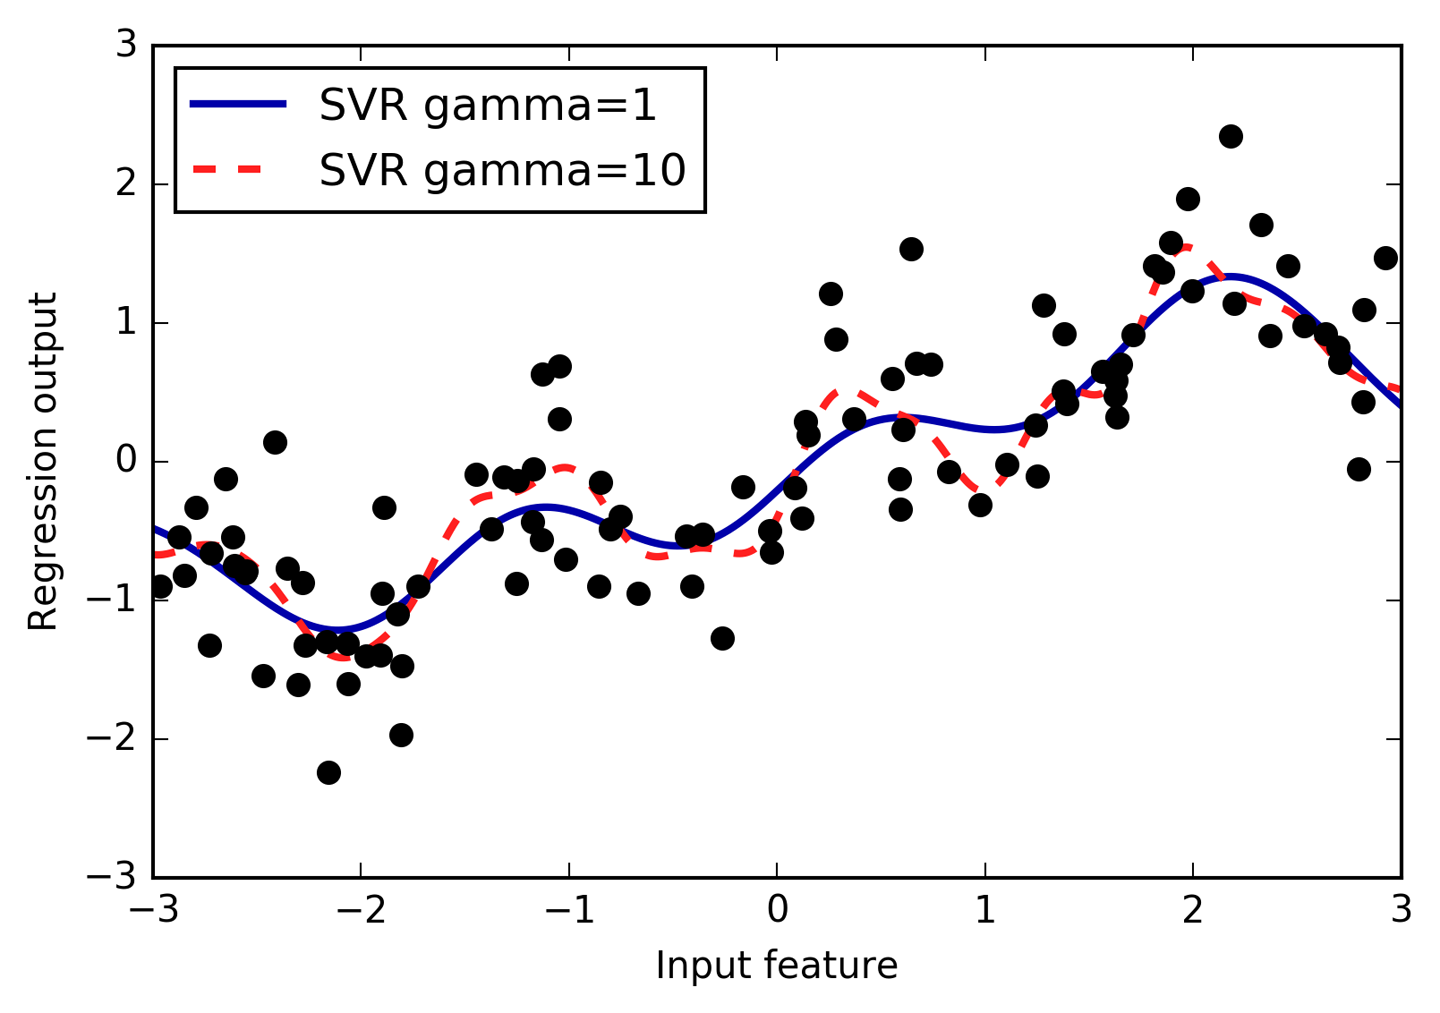
\includegraphics[width=0.45\textwidth]{gamma}
\end{figure}
You can find detailed information about C and gamma params in sklearn library documentation\cite{rbf_params}.

\subsection{K-nearest Neighbors Regression}

Another, examined algorithm used to estimating time of a module execution is a simple \textit{KNN}\footnote{\textit{KNN} - k-nearest neighbors} regression. Using the algorithm, a target is predicted by local interpolation of the targets associated of the nearest neighbors in the training set~\cite{knnreg}.In another words, the target assigned to a query point is computed based on the mean of the targets of its nearest neighbors.

To use the algorithm we have to define values of the following parameters:
\begin{enumerate}
	\item \textit{k} - number of the nearest neighbors
	\item \textit{weights} - weight function used in prediction. The basic nearest neighbors regression uses uniform weights: that is, each point in the local neighborhood contributes uniformly to the classification of a query point. Under some circumstances, it can be advantageous to weight points such that nearby points contribute more to the regression than faraway points. The weights can be calculated from the distances using any function for example the linear one.
	\item \textit{algorithm} - the procedure to calculate k-nearest neighbors for the query point. It does not have a direct impact to the final regression result, but the parameters of the algorithm surely have. For example, using the BallTree algorithm we have to choose the \textit{metric} parameter that will be used to calculate the distance between data points. It could be, for example, the Minkowski~\cite{minkowski} metric with the l2 (standard Euclidean~\cite{euclidean}) distance metric or any function that will calculate the distance between two points.
\end{enumerate}

\begin{figure}[!htb]
	\caption{KNN out of range fail.}
	\centering
	\label{fig:knn}
	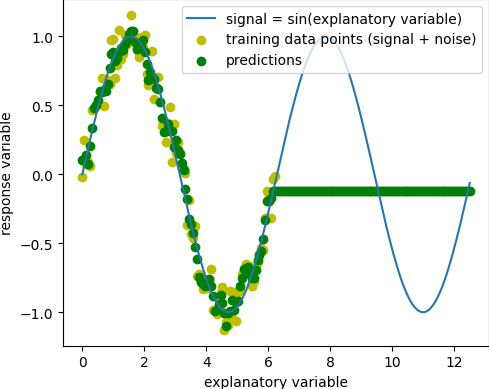
\includegraphics[width=0.45\textwidth]{knn}
\end{figure}